%!TEX root = main.tex
%%%%%%%%%%%%%%%%%%%%%%%%%%%%%%%%%%%%%%%%%%%%%%%%%%%%%%%%%%%%%%%%%%%%%%%%%%%%%%%%%%%%%%%%%%%%%%%%%%%%%%
%
%   Filename    : appendix_A.tex 
%
%   Description : This file is one of the appendices. 
%                 
%%%%%%%%%%%%%%%%%%%%%%%%%%%%%%%%%%%%%%%%%%%%%%%%%%%%%%%%%%%%%%%%%%%%%%%%%%%%%%%%%%%%%%%%%%%%%%%%%%%%%%

\chapter{Research Ethics Forms}
\label{sec:appendixa}

\chapter{Turnitin Similarity Report}
\label{sec:appendixb}

% \chapter{Data Collection Artifacts}
% \label{sec:appendixc}

\chapter{Design Artifacts}
\label{sec:appendixd}

\section{Affinity Diagram}

\newpage
\section{User Personas}
\label{sec:user-personas}

\begin{wrapfigure}{l}{0.5\textwidth}

  \begin{center}
    
\includegraphics[width=0.48\textwidth]{mary_persona}
  \end{center}
\end{wrapfigure}


Mary: The Amateur \newline

\begin{itemize}
\item 18 years old
\item Started composing as a hobby when she was 16 years old
\item 2nd Year undergraduate student
\item Currently taking up a Bachelor in Music degree program
\item Passing grades during her 1st Year
\end{itemize}

"Its such a hassle to write notes on music sheets. Its hard to keep track which are the drafts."

"I haven't found any app like Finale in the app store."

Mary lives in a dorm with 3 other people and has her own laptop and tablet. She uses both of these devices to do her work in any place.

Mary mostly uses music sheets when she needs to compose music for assignments. She usually uses her laptop for research and the tablet as a substitute when she doesn't feel like bringing her laptop.

Mary has passing marks in her courses. She experiences difficulty getting high grades because she has a hard time looking for inspiration and ideas. She also easily gets tired writing, revising, and finalizing her compositions on paper.

She is knowledgeable in using Sibelius on her laptop and has started to learn Finale due to her professors urging her to use it. She appreciates how these kinds of applications reduce the steps in some repetitive or tedious processes in composing music. \newline

\begin{wrapfigure}{l}{0.5\textwidth}
  \begin{center}
  
    
\includegraphics[width=0.48\textwidth]{warren_persona}
  \end{center}
\end{wrapfigure}

Warren: The Experienced \newline

\begin{itemize}
\item 34 years old
\item 10 years of composing music professionally
\item Music teacher in a high school
\item Loves classical music
\item Music fundamentalist
\item Wants his students to be more engaged in music and appreciate the art form
\item Faculty for 5 years
\end{itemize}

"Music is a way to truly express yourself"

"I want to share my passion in music to my pupils"

Warren is currently a faculty member of a private high school that pays him enough that he can make a living and support his family.

Warren has been teaching for 5 years. He has been involved in organizing the curriculum in the school. He has always believed that music as an art form is timeless and should be learned by everyone.

He wants his students to appreciate music as much as he does. He shares the works of Beethoven and Mozart, which are his favorites, to his class.

% He wants his students to appreciate music since years of hard work from various authors like Beethoven and Mozart have devoted their whole lives to the art. 

He often observes students using their mobile devices in school. During class, he's made it clear that the usage of cellphones is restricted. However, he understands the potential of these mobile devices as tools for musical composition.

% He often observes students being too distracted with their devices in school. During class, he's made it clear that the usage of cellphones is restricted. Though, he can see the usefulness of the technology for research and some classes in his school has integrated e-learning.

He is experienced in using Finale but still uses music sheets during occasions where he cannot use his laptop or is still sketching. He has been wondering whether there is a viable mobile alternative to using music sheets. \newline

% He's been wondering if these technologies can be used for teaching music but he's on the fence about it because students might not experience music fully.



\begin{wrapfigure}{l}{0.5\textwidth}
  \begin{center}
    
\includegraphics[width=0.48\textwidth]{winston_persona}
  \end{center}
\end{wrapfigure}

Winston: The Veteran \newline

\begin{itemize}
\item 62 Years Old
\item 40 years of experience in composing music professionally
\item Composes music for different companies and artists
\item Mentors up and coming composers
%\item Active in international conferences about the field of Music
\item Married for 35 years
\item Has experienced the numerous shifts of popularity between music genres
\end{itemize}

"Music has always been a part of everyone's lives" 

"I wonder whats next the next big thing that can change music" 

Warren always reads on music-related news and enjoys doing research on topics that concern music. He writes his findings and his thoughts on his blog. He has lived through several shifts in mainstream music and has studied the change agent in every shift. 

He has been able to adjust and make a living from these hobbies. He has always been able to make music that matched what was popular at the time. He fully accepts that music changes for every new generation of artists and composers.

He is waiting for the next big thing that can happen for music, always prepared to make the needed adjustments to stay in the game. He is no stranger to using technology like Finale or Sibelius to compose his pieces.

\begin{comment}
\chapter{Resource Persons}
\label{sec:appendixf}

\newcommand{\resperson}[4]{\textbf{#1} \\ #2 \\ #3 \\ \url{#4}\vspace{0.5em}\\}

\resperson{Mr. Jordan Aiko Deja}{Adviser}{College of Computer Studies\\De La Salle University-Manila}{jordan.deja@dlsu.edu.ph}
\\
\resperson{Dr. Rafael Cabredo}{Chair, Software Technology Department}{College of Computer Studies\\De La Salle University-Manila}{rafael.cabredo@dlsu.edu.ph}

\end{comment}

\chapter{Literature Map}
\label{sec:appendixe}


\begin{sidewaysfigure}[h]
    %\centering
	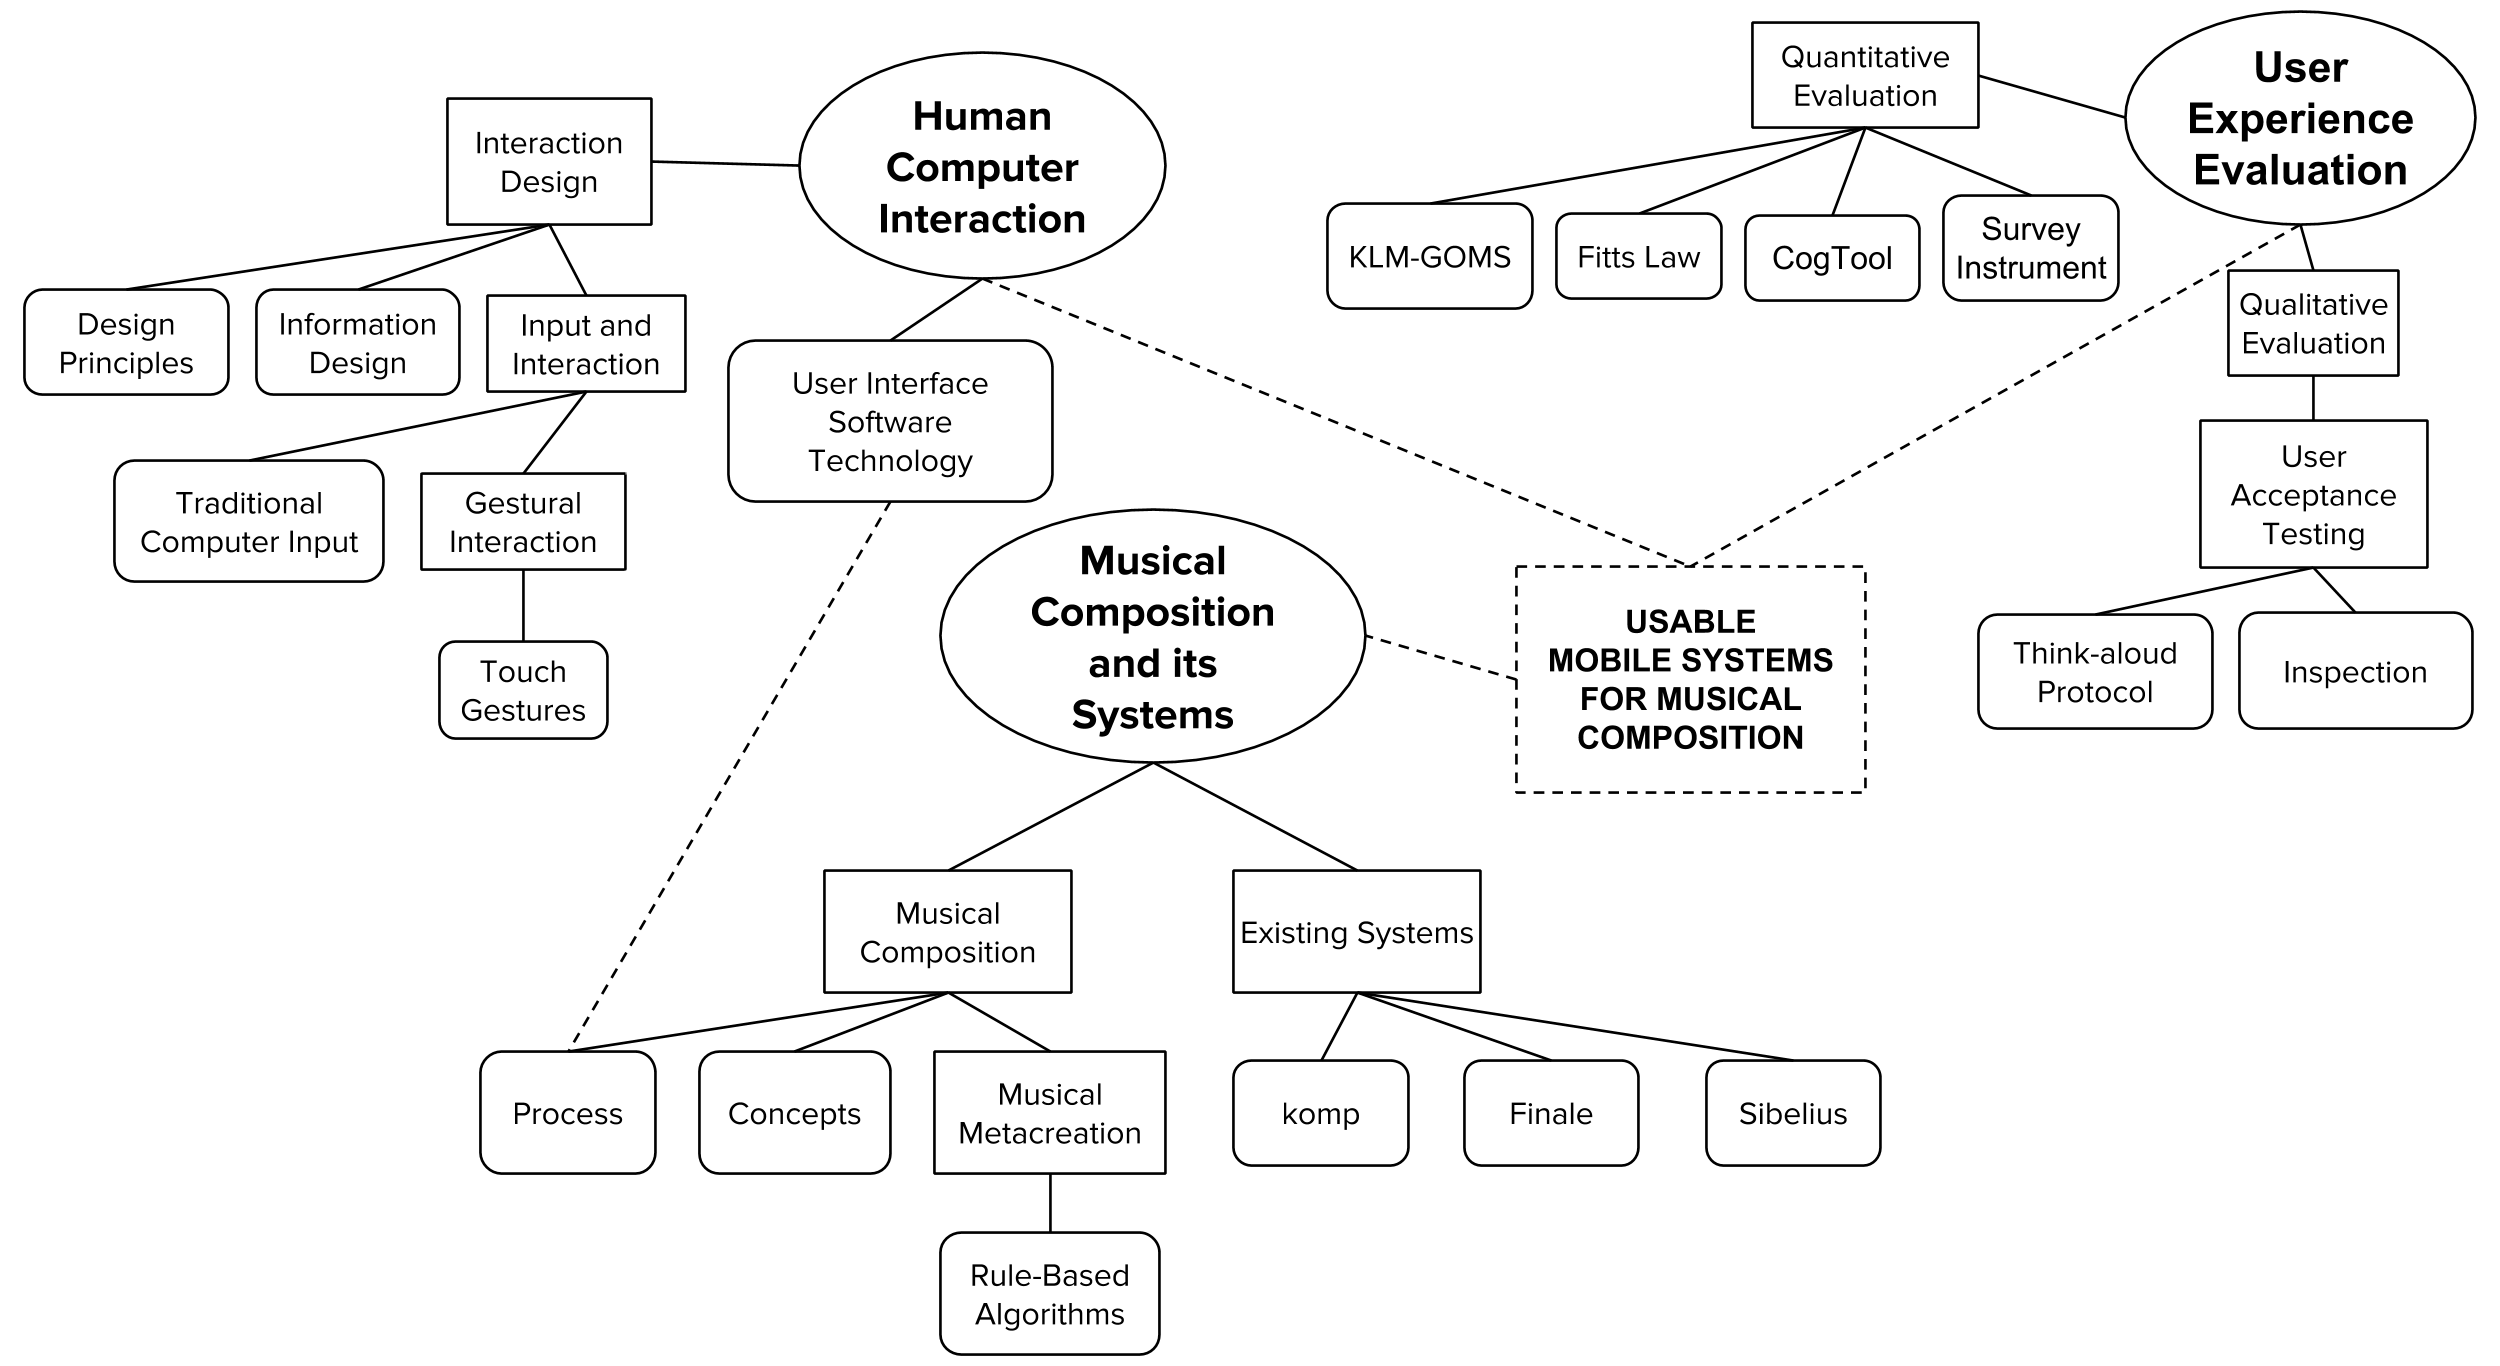
\includegraphics[scale=0.26]{literature_map}
    \caption{Literature map.}
    \label{fig:literature-map}
\end{sidewaysfigure}

\begin{comment}
\chapter{Initial Results}
\label{sec:appendixf}

\begin{longtable}{|p{5cm}|p{6cm}|p{1.5cm}|}
\caption{Motor Module} \label{tab:motor-module} \\
\hline

Attribute & Attribute Description & Value \\ \hline

PECK-FITTS-COEFF & b coefficient in Fitts's equation for PECK movements. & 0.075 \\ \hline

DEFAULT-TARGET-WIDTH & Effective width, in degrees visual angle, of targets with undefined widths. & 1.0 \\ \hline

MIN-FITTS-TIME & Minimum movement time for an aimed [Fitts's] movement. & 0.1  \\ \hline

MOTOR-BURST-TIME & Minimum time for any movement. & 0.05 \\ \hline

MOTOR-INITIATION-TIME & Time to initiate a motor movement. & 0.05 \\ \hline

MOTOR-FEATURE-PREP-TIME & Time to prepare a movement feature. & 0.001 \\ \hline

\end{longtable}

\begin{longtable}{|p{5cm}|p{6cm}|p{1.5cm}|}
\caption{Imaginal Module} \label{tab:imaginal-module} \\
\hline

Attribute & Attribute Description & Value \\ \hline

IMAGINAL-DELAY & Time in seconds to respond to an imaginal request & 0.2 \\ \hline

\end{longtable}

\begin{longtable}{|p{5cm}|p{6cm}|p{1.5cm}|}
\caption{Temporal Module} \label{tab:temporal-module} \\
\hline

Attribute & Attribute Description & Value \\ \hline

TIME-NOISE & Temporal noise & 0.015 \\ \hline

TIME-MASTER-START-INCREMENT & Temporal start interval & 0.011 \\ \hline

TIME-MULT & Temporal multiplier & 1.1 \\ \hline

RECORD-TICKS & Record each time increment as a buffer event & T \\ \hline

\end{longtable}

\end{comment}